\documentclass[11pt]{article}


%%% Packages
%%
\usepackage{amsmath}
\usepackage{amsfonts}
\usepackage{amssymb}
\usepackage{fancyhdr}
\usepackage{float}
\usepackage{graphicx}
\usepackage{listings}
\usepackage{enumitem}
\usepackage[margin = 1in, headheight = 13.6pt]{geometry}
\usepackage[linktoc=all]{hyperref}
%%
%%%


%%% Formatting
%%
\parindent 0em
\parskip 1em
\pagestyle{fancy}
\fancyhead{}
\fancyfoot{}
\fancyhead[L]{\slshape\MakeUppercase{{\myTitle}}}
\fancyhead[R]{\slshape{\myName}}
\fancyfoot[C]{\thepage}
%%
%%%


%%% User defined variables
%%
\def \myTitle {ECE 404 Homework 8}
\def \myName {Elias Talcott}
\def \myDate {March 26, 2020}
%%
%%%


\begin{document}

\begin{titlepage}
\title{\myTitle}
\author{\myName}
\date{\myDate}
\maketitle
\vspace{1in}
\tableofcontents
\thispagestyle{empty}
\end{titlepage}


\section{Port Scanning}

This image shows a portion of the result when port scanning was performed on IP address 192.168.1.1 using IP address 192.168.1.20. Most ports shown in this image are closed, but port 53 is detected to be open. The port scan from port 0 to port 1000 took approximately a minute and a half.

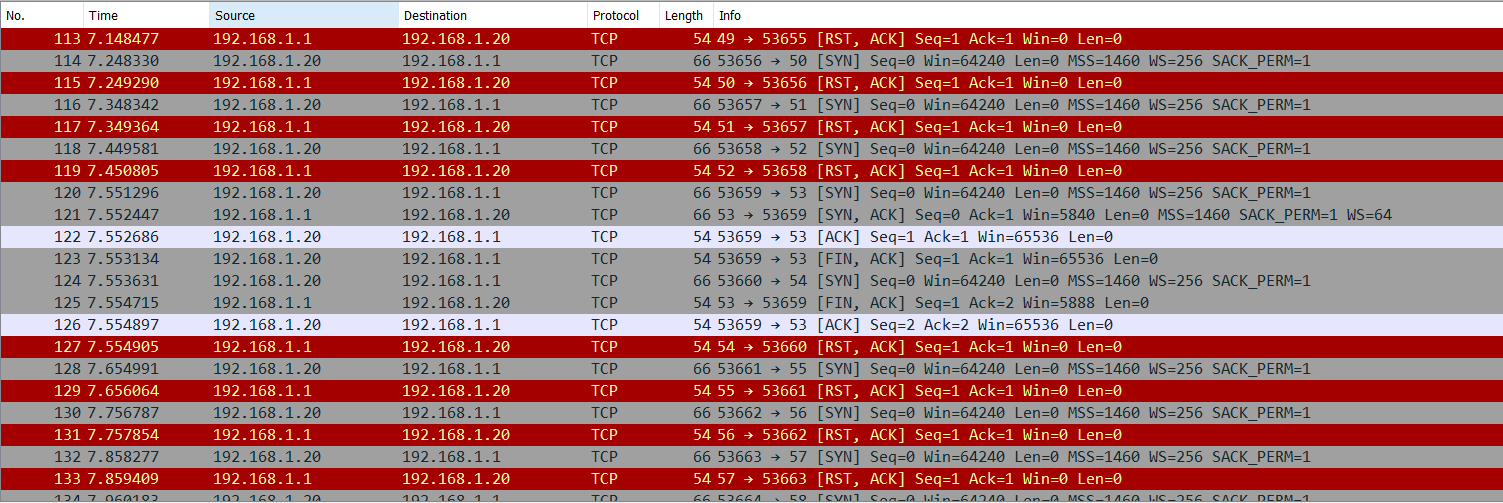
\includegraphics[width=\linewidth]{PortScanning.png}

\section{SYN Flood Attack}

This image shows a portion of the result of a SYN flood attack performed on IP address 192.168.1.1 using the spoof IP address 192.168.1.50. The source port is a randomly generated integer between 1024 and 65536 (non-"well-known" ports) and the destination port and number of SYN packets sent are as specified in the method call. 

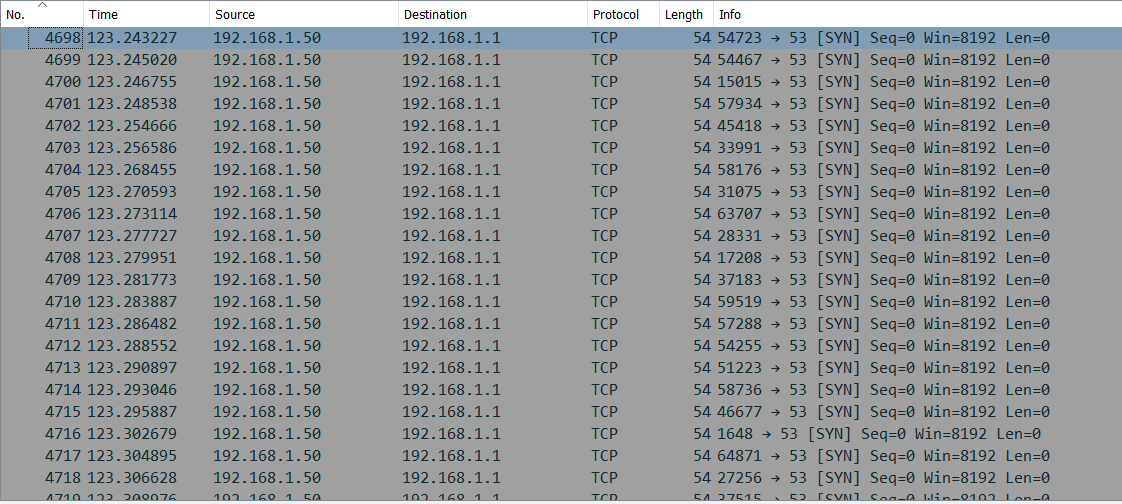
\includegraphics[width=\linewidth]{SYNFlood.png}

\end{document}